%% Los margenes, tipo de hoja y estilo BOOK
\documentclass[a4paper,11pt,twoside,openright,titlepage]{book}
\usepackage[a4paper,left=1in,right=1in,top=0.6in]{geometry}

\usepackage[T1]{fontenc}    %Ineterprete de tíldes
%\usepackage[Latin1]{inputenc}
\usepackage{amsmath,amssymb}    %Paquete de entornos matematicos

\usepackage{natbib}
\usepackage[english,spanish]{babel}
\selectlanguage{spanish} 
\usepackage{graphicx}
\usepackage{psfrag}
\usepackage{quotchap}
\usepackage{epsfig}
\usepackage[all]{xy}
\usepackage[utf8]{inputenc}
\usepackage{epsfig}
\usepackage{makeidx}
\usepackage{ifthen}
\usepackage{multicolpar}    %Para poner texto en columnas en plan articulo intercalado con texto normal
\usepackage{multicol,multirow}

\usepackage{url}        %Para direcciones web
\usepackage{marvosym}   %Para imprimir el simbolo de \EUR euro
%\usepackage{eurosym}   %Para imprimir el simbolo de \euro euro
\usepackage{fancybox}   %Para tablas con bordes redondeados


%% Modificación de la plantilla para adaptarla a los requisitos de PFC
\usepackage{fancyhdr}
\pagestyle{fancy}
%%% Cabeceras y pies de página
\fancyhead[CE,CO]{\emph{\titulo}}
\fancyhead[LE,LO,RE,RO]{}
\fancyfoot[LE,RO]{\thepage}
\fancyfoot[CE,CO]{\leftmark}

\renewcommand{\footrulewidth}{.6pt}


%Definiciones de funciones para los titulos
\newlength\salto
\setlength{\salto}{3.5ex plus 1ex minus .2ex}

\newlength\resalto
\setlength{\resalto}{2.3ex plus.2ex}

\newcommand{\lsection}[1]
                {\section{#1}
                \vskip-.9\resalto   %%%% Aquí reculo el posible salto por defecto de \section
                \hrule
                \vskip+.9\salto}  %%%% vuelvo ha realizar el salto (puedes poner otra vez el 90%)


%Para imágenes de entornos estáticos \captionFigure{Texto Caption}{Texto Label}
\newcommand{\captionFigure}[2]{
    \refstepcounter{figure}
    \centerline{Figura \thefigure: #1 \label{#2}}
    \addcontentsline{lof}{section}{\thefigure.\ #1\label{#2}}
}

%Para imágenes de entornos estáticos \NOcaptionFigure{Texto Caption}{Texto Label} "No escribe el caption"
\newcommand{\NOcaptionFigure}[2]{
    \refstepcounter{figure}
    \addcontentsline{lof}{figure}{\thefigure.\ #1\label{#2}}
}


%% Datos del PFC

\newcommand{\titulo}{1718\_072\_IC \- Diseño e implementación de un hub de control domótico}
\newcommand{\autor}{Autor: Pallarés Jiménez, Ignacio}
\newcommand{\director}{Nombre Apellido1 Apellido2}
\newcommand{\tutor}{Tutor: Delgado Mohatar, Óscar}
\newcommand{\ponente}{Ponente: Anguiano Rey, Eloy}
\newcommand{\vocal}{Nombre Apellido1 Apellido2}
\newcommand{\vocalsup}{Nombre Apellido1 Apellido2}
\newcommand{\presidente}{Nombre Apellido1 Apellido2}
\newcommand{\presidentesup}{Nombre Apellido1 Apellido2}
\newcommand{\fecha}{JULIO 2018}
\newcommand{\carrera}{Grado en Ingeniería Informática}

\begin{document}
\setlength{\baselineskip}{18pt}  %% Espacio interlinea
\setlength{\parskip}{6pt plus 1pt minus 1pt} %% Espacio interpárrafo

\begin{titlepage}

\begin{center}

\vspace*{2cm}

\LARGE \textsc{Universidad Autónoma de Madrid}\\

\vspace{.2cm}

\large \textsc{Escuela politécnica superior}\\

\vspace{.2cm}

\begin{figure}[h]
    \begin{center}
        \begin{minipage}[c]{0.495\linewidth}
            \rightline{\epsfig{figure=images/logo_eps.eps,width=0.5\linewidth}}
        \end{minipage}
        \begin{minipage}[c]{0.495\linewidth}
            \leftline{\epsfig{figure=images/logo_uam.eps,width=0.5\linewidth}}
        \end{minipage}
    \end{center}
    \label{fig:Escudos}
\end{figure}

\Huge \carrera\\

\vspace{1cm}

\Huge \textsc{Trabajo Fin de Grado}\\

\vspace{1.5cm}

\Huge \MakeUppercase{\textbf{\titulo}}

\vspace{3cm}


\Large \autor\\
\Large \tutor\\
\Large \ponente\\

\vspace{0.5cm}

\Large \fecha

\end{center}

\end{titlepage}

\normalsize


\newpage \thispagestyle{empty} % Página vacía


\frontmatter %Define el cuerpo inicial del libro en numeración con letras romanas

\chapter*{}

\vspace*{0.2cm}

\begin{center}

\Huge \MakeUppercase{\textbf{\titulo}}

\vspace{7cm}

\Large \autor \\
\Large \tutor \\
\Large \ponente \\

\vspace{5cm}


Grupo de la EPS (opcional) \\
Dpto. de XXXXX \\
Escuela Politécnica Superior \\
Universidad Autónoma de Madrid \\
\fecha

\end{center}

\normalsize

\newpage \thispagestyle{empty} % Página vacía


\chapter*{Resumen}

\section*{Resumen}

La domótica consiste en la automatización del hogar. Los sistemas domóticos, son aquellos capaces de domotizar una vivienda; proporcionan servicios de comunicación,
seguridad, eficiencia energética...etc. Sin duda alguna, la comunicación entre estos sistemas es algo esencial, existiendo redes cableadas e inalámbricas para ello, pudiendo
ser controlados estos sistemas desde dentro y fuera del hogar.

BRIMO es un proyecto de código abierto para la gestión y el control de dispositivos domóticos en el hogar. Es una alternativa open source de bajo coste para todas
aquellas personas que deseen domotizar su hogar de una manera barata y sencilla. No utiliza protocolos privados, y cualquiera que lo desee puede utilizar y modificar
la aplicación a su gusto.

Además, cualquier persona puede crear sus dispositivos (sensores, actuadores o cámaras) de manera sencilla, siempre que éstos sigan los requisitos establecidos.
Brimo nos ayuda, gracias a una interfaz sencilla e intuitiva, a ordenar nuestros dispositivos, visualizar sus estados y mandar comandos a los dispositivos que los acepten.

La aplicación está pensada para ejecutarse en entornos ligeros, concretamente en una Raspberry Pi 3 (precio asqequible), pero también puede ser ejecutada en cualquier ordenador tras una simple configuración.
Utiliza una arquitectura REST sobre el protocolo HTTPS para comunicarse con los dispositivos.

La función principal de Brimo es de "bridge", punto común entre el usuario y los dispositivos, se encarga de poner en contacto al usuario con los dispositivos.
\section*{Palabras Clave}
Domótica, código abierto, REST, raspberry, HTTP, sensores, MVC, actuadores, bridge.
\newpage

%-------------------------------------------------------------------------------------------------------------------------------------

\section*{Abstract}
Domotic consists of home automation. Domotic systems are those capable of automating a home; providing communication services,
security, energy efficiency ... etc. Communication between these systems is essential, existing wired and wireless networks for it,
that allows us to controll them from inside and outside the home.

BRIMO is an open-source project for the management and control of domotic devices in the home. It is a low-cost open source alternative for all people
 who want to domotize their home in a cheap and simple way. It does not use private protocols, and anyone can use or modify the application on its preferences.

Besides, anyone is able to create its own devices (sensors, actuators or cameras) in a simple way, following the application requirements. Brimo helps us, thanks to
a simple and intuitive interface, to arrange our devices, seeing their status and to send them commands.

The application is designed to be runned on lightweight devices, specifically into a Raspberry Pi 3 (low cost), but it could be also runned on any computer after a simple
configuration. It uses REST architecture over HTTPS protocol to communicate with devices.

The main function of Brimo is to act as bridge, the common point between users and devices: Brimo is the responsible of the communication between them.
\section*{Key words}

Domotic, open-source, low cost, REST, raspberry, HTTP, sensors, MVC, actuators.

\chapter*{Agradecimientos}


\tableofcontents

\newpage \thispagestyle{empty} % Página vacía

\addcontentsline{toc}{chapter}{Índice de Figuras}    %Para que aparezca en el índice
\renewcommand{\listfigurename}{Índice de Figuras} 
\listoffigures

\newpage \thispagestyle{empty} % Página vacía

\addcontentsline{toc}{chapter}{Índice de Tablas}    %Para que aparezca en el índice
\renewcommand{\listtablename}{Índice de Tablas} 
\listoftables

\newpage \thispagestyle{empty} % Página vacía

\mainmatter %Define el cuerpo principal del libro numeración normal.

% \input{preambulo}

\chapter{Introducción} 
\label{chap:intro}

\vspace{-0.2cm}

\lsection{Motivación del proyecto}

Los sistemas domóticos por lo general utilizan una arquitectura centralizada: un controlador (bridge) es el encargado de enviar y recibir información de los dispositivos domóticos y las interfaces.
 Se utilizan sistemas centralizados debido a que abaratan mucho el coste de los dispositivos domóticos, así los dispositivos tienen poca electrónica y programación, y la responsabilidad principal
 reside en el bridge. Este enfoque tiene sentido cuando se trata de muchos dispositivos en un hogar, que es el caso ideal, si solo tuviésemos un sensor carecería de sentido tener un sensor y un bridge para manejarlo.

El problema principal que existe con los sistemas centralizados se encuentra en la \textbf{compatibilidad} entre dispositivos y bridges.
Por lo que he observado~\cite{article:EstadoDelArte}, todavía falta mucha estandarización en el
ámbito de la domótica: cada fabricante usa sus medios y protocolos haciendo incompatibles bridges y dispositivos. Además, estos dispositivos no suelen ser 
muy asequibles. Por lo tanto, nos encontramos ante la necesidad de comprar todos los dispositivos de una misma marca o tener muchos bridges, lo que nos obligaría a manejar cada
dispositivo desde su correspondiente bridge.

La domótica puede hacernos la vida en el hogar mucho más sencilla, ayudándonos a ahorrar tiempo y dinero que podremos invertir en otras cosas. Los hogares todavía están muy poco automatizados, y mi principal motivación ha sido acercar la domótica 
a las personas y aprender acerca de ella. Gracias a nuestro sistema manejamos todos los dispositvos a través de un solo bridge de manera sencilla y eficaz.

\newpage
\lsection{Objetivos y enfoque}

El objetivo último de nuestro proyecto es desarrollar un sistema que sea capaz de recibir y enviar información de dispositivos domóticos y sea capaz de interactuar con el cliente. 

Los \textbf{requisitos} que debe cumplir nuestro sistema son:
\begin{itemize}
  \item \underline{Ligero.} Un bridge no debería necesitar demasiada capacidad de procesamiento y de memoria, y es necesario que no sea muy costoso, por lo tanto, la ligereza es requisito indispensable.
  \item \underline{Compatibilidad.} Necesitamos que nuestro bridge no sea únicamente compatible con un tipo de sensor, o un modelo de cámara
  \item \underline{Interfaz sencilla y adaptable a cualquier dispositivo.} Necesitamos que la interfaz de nuestro bridge sea compatible con cualquier dispositivo sin perder funcinalidad.
  \item \underline{Seguridad.} La seguridad en la domótica es algo indispensable, confío en que el día de mañana incluso las cerraduras de nuestras casas serán automáticas, y no podemos dejar la responsabilidad de la seguridad
  de nuestra a casa a un sistema con vulnerabilidades de seguridad.
  \item \underline{Escalable.} Nuestro sistema ha de ser escalable y debemos pensar en todo momento en ampliaciones y trabajos futuros. La domótica evoluciona a pasos agigantados y podríamos añadir funcionalidades a nuestro 
  sistema practicamente a diario. No obstante, es necesario acotar firmemente los límites de nuestro proyecto para ceñirnos a las horas que corresponden a un TFG, aunque debemos tener muy en cuenta en todo momento trabajos futuros y ampliaciones.
  Además, debemos tener en cuenta la escalabilidad: domótica en un hospital, en una ciudad...etc.
\end{itemize}


\lsection{Metodología y plan de trabajo}

Debido a que los capítulos del documento coinciden con las fases de ciclo de vida de nuestro proyecto, es importante explicar la metodología antes de explicar la estructura del documento.
\par
La metodología que se ha utilizado para el desarrollo de nuestro proyecto es una metodología tradicional con un ciclo de vida en cascada. Se utilizarán las siguientes etapas, que se realizarán una detrás de otra (en cascada):

\begin{figure}[H]
\centering
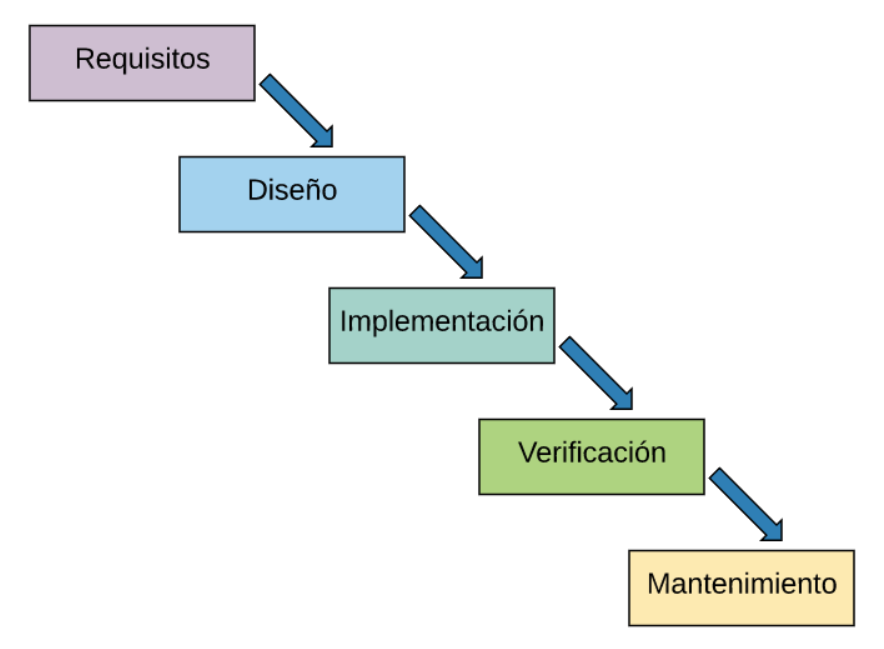
\includegraphics[width=5.00in]{images/desarrollo_cascada.PNG}
\caption{Las etapas del modelo en cascada.
 Recuperado de: https://openclassrooms.com/en/courses/4309151-gestiona-tu-proyecto-de-desarrollo/4538221-en-que-consiste-el-modelo-en-cascada}
\label{fig:tecnologias_populares}
\end{figure}

\lsection{Estructura del documento}

A lo largo del siguiente documento se irán explicando todas las fases del ciclo de vida de nuestro proyecto, además de tener una fase previa de análisis de estado del 
arte y una fase posterior de trabajos futuros y conclusiones:
\begin{itemize}
\item\textbf{Estado del arte - \autoref{chap:estadodelarte}}: breve introducción y análisis de la domótica en la actualidad.
\item\textbf{Análisis y diseño - \autoref{chap:analisisydisenosistema}}: a lo largo del capítulo tres se analizan los requisitos de nuestra aplicación y se diseña la arquitectura del sistema.
\item\textbf{Desarrollo del sistema - \autoref{chap:desarrollosistema}}: en este capítulo se describirán las tecnologías utilizadas para el desarrollo del sistema, y se detallarán 
algunos aspectos técnicos acerca de la implementación.
\item\textbf{Pruebas - \autoref{chap:pruebas}}: en este capítulo se detallarán las pruebas realizadas para comprobar el correcto funcionamiento
de nuestro sistema y la detección de posibles bugs.
\item\textbf{Trabajos futuros - \autoref{chap:trabajofuturo}}: análisis de posibles trabajos futuros para nuestro HUB.
\item\textbf{Conclusiones - \autoref{chap:conclusiones}}: conclusiones obtenidas a lo largo del trabajo.
\end{itemize}


\newpage \thispagestyle{empty} % Página vacía 

\chapter{Estado del arte}
\label{chap:estadodelarte}

\lsection{Introducción}

\lsection{Historia, nacimiento y evolucin.} \label{sec:historia}

\lsection{La anatoma del ojo}
\label{sec:anatomiaojo}
\subsection{Aspectos diferenciadores del iris}


\lsection{Adquisicin del Iris} \label{sec:adquisicion}
\subsection{Introduccin}
\subsection{Esquemas de adquisicin tradicionales}
\subsection{Consideraciones sobre la iluminacin}
\label{subsec:iluminacion}
\subsection{Posicionamiento del Iris}
\subsection{Sistemas comerciales de adquisicin}


\lsection{Localizacin y segmentacin del Iris} \label{sec:localizacion}
\subsection{Introduccin}
\subsection{Metodologa de J. Daugman y derivadas}
\subsection{Metodologa de R. Wildes y derivadas}
\subsection{Otras metodologas}
\subsection{Comparativa de metodologas}
\subsection{Deteccin de pestaas y ruido}


\lsection{Normalizacin del tamao}
\label{sec:normalizacion}
\subsection{Daugman's Rubber Sheet Model}
\subsection{Image Registration}
\subsection{Normalizacin en ngulo}
\subsection{Mejora del contraste y eliminacin de ruido}


\lsection{Algoritmos de Codificacin}
\label{sec:codificacion}
\subsection{Metodologa de Daugman: Filtros de Gabor}
\subsection{Metodologas alternativas a la de Daugman}
\subsubsection{Filtros Log-Gabor} \label{subsubsec:filtrosLogGabor}
\subsubsection{Wavelets}
\subsubsection{Haar Wavelet}
\subsubsection{Transformada Discreta del Coseno (DCT)}
\subsection{Metodologas de Wildes. Vectores de caractersticas reales (no binarios)}


\lsection{Algoritmos de Matching}
\label{sec:matching}
\subsection{Introduccin}
\subsection{Distancia de Hamming} 
\label{subsec:distHamming}
\subsection{Distancia eucldea ponderada}
\subsection{Correlacin normalizada}


\lsection{Problemtica y retos futuros}
\label{sec:problematica}
\subsection{Segmentacin}
\subsection{Captura ideal no invasiva}


\lsection{Competiciones o Evaluaciones de Iris}
\label{sec:competiciones}
\subsection{The Iris Challenge Evaluation (ICE)}
\subsection{The Noisy Iris Challenge Evaluation (NICE)}


\lsection{Bases de datos} \label{sec:databases}
\subsection{CASIA} \label{sec:CASIA_database}
\subsection{BioSec Baseline y BioSecurID} \label{sec:ATVS_database}



\newpage \thispagestyle{empty} % Pgina vaca 

\chapter{Sistema, diseño y desarrollo}
\label{chap:sistemadesarrollado}

\lsection{Segmentacin}

\lsection{Normalizacin}

\lsection{Codificacin}

\lsection{Matching}


\chapter{Protocolos}
\label{chap:experimentos}

Este capítulo esta dedicado a describir los protocolos utilizados en este proyecto, apoyados sobre HTTP e implementados con un servidor CherryPy.
El back-end de nuestro bridge va a diferenciar entre dos tipos de comunicación: comunicación directa con los dispositivos y comunicación con el front-end de la interfaz.

\lsection{Comunicación con los dispositivos} \label{sec:ProtocolosDispositivos}

En esta sección se describirá la comunicación con los dispositivos: registro de dispositivos y actualización de la información. El sentido de la comunicación es dispositivo -> bridge, y todos los tipos de dispositivos 
siguen este protocolo.

\begin{table}[h]
    \centering
    \scriptsize
    \begin{tabular}{|l|l|l|l|}
    \hline
        MÉTODO & ENDPOINT    & DESCRIPCION                                                & SEGURIDAD \\ \hline
        POST    & /devices/register    & Registra un nuevo dispositivo.            & NO     \\ \hline
        PUT    & /device/:id & Edita la información de un dispositivo.                              & NO     \\ \hline
    \end{tabular}
\end{table}

\subsection{Registro de nuevos dispositivos} \label{sec:RegistroDispositivos}

La primera vez que un dispositivo se conecta al bridge es necesario que realice una primera llamada de registro. De esta manera, el bridge dará de alta el dispositivo
y sabrá de qué tipo de dispositivo se trata.



\chapter{Experimentos Realizados y Resultados}
\label{chap:experimentos}

\lsection{Bases de datos y protocolo}

\lsection{Sistemas de referencia}
\label{sect:sistemasreferencia}

\lsection{Escenarios de pruebas}
\label{sect:escenarios_pruebas}
 
\lsection{Experimentos del sistema completo}


\chapter{Conclusiones y trabajo futuro}
\label{chap:conclusiones}


\newpage \thispagestyle{empty} % Página vacía 

\chapter*{Glosario de acrónimos}
\addcontentsline{toc}{chapter}{Glosario de acrónimos}

\begin{itemize}
  
\item{\textbf{Sistema domótico}: Un sistema domótico es el conjunto de controladores y dispositvios que hacen posible la automatización del hogar.}
\item{\textbf{Dispositivo domótico}: Dispositivo que nos ayuda a la automatización del hogar actuando o recopilando información. Ejemplos: sensores de temperatura, relés, cámaras...etc. }
\item{\textbf{Bridge}: Dispositivo que nos ayuda a controlar y administar diferentes dispositivos domóticos. Los dispositivos se conectan al bridge, y el cliente interactua directamente a través de él. }
\item{\textbf{REST}: Arquitectura software que se apoya en el protocolo HTTP. Se utiliza en arquitecturas cliente-servidor. El cliente tiene operaciones básicas y predefinidas: GET, POST, PUT, DELETE... Y el sevidor responde a las peticiones con su correspondiente código HTTP.
Cada recurso del servidor es direccionable a través de su URI.}
\item{\textbf{Angular5}: Framework de código abierto mantenido por Google para la creación y mantenimiento de Single Page Applications (SPA). Desarrollado en TypeScript. }
\item{\textbf{SPA}: Del inglés Single Page Application: aplicación web que se ejecuta en una sola página, sin necesidad de refrescar el navegador, haciendo más fluida la navegación.}
\item{\textbf{MVC}: Modelo Vista Controlador: arquitectura software que separa los datos (Modelo) de la interfaz de usuario (Vista), su comunicación y lógica se encuentra en el controlador.}
\item{\textbf{Responsive}: Diseño web cuyo objetivo es adaptar la apariencia de la página web a diferentes dispositivos.}
\item{\textbf{Ataque Man-In-The-Middle}: Tipo de ataque en el que el atacante es capaz de interceptar y/o modificar mensajes enviados entre dos partes. 
Comúnmente este ataque se realiza en redes donde se utilizan protocolos HTTP, el atacante es capaz de captar las peticiones y modificarlas.}
\end{itemize}

\newpage \thispagestyle{empty} % Página vacía

\addcontentsline{toc}{chapter}{Bibliografa}    %Agregamos al ndice el capitulo de bibliografa 

\bibliographystyle{unsrt}   %plain pero ordenado en orden de aparacicion en documento principal
\bibliography{bibliografia}

\appendix   %Indicamos que lo que viene a continuación son apéndices

%\frontmatter %Para poner los anexos en numeros romanos

\chapter{Manual de utilización}
\label{Anexo:manualuso}


\newpage \thispagestyle{empty} % Página vacía 

\chapter{Manual del programador}
\label{Anexo:codigosMatlab}


\newpage \thispagestyle{empty} % Página vacía 

%Hoja final en blanco
\newpage \thispagestyle{empty} % Página vacía

\end{document}
